\newpage
\section{Prezentacja aplikacji}
\vspace{1cm}
    Aplikację mobilną podzielić można na dwa główne widoki. Pierwszy, z którym zetknie się użytkownik, to ekran autoryzacji. Tam możliwe jest dla niego stworzenie nowego konta lub zalogowanie się
    na istniejące już konto. Drugi to ekran główny, w którym odbywają się wszystkie kluczowe aktywności związane z głównym celem aplikacji, jakim jest stworzenie narzędzia do dzielenia się 
    ciekawymi miejscami i planami wycieczek.

\vspace{1cm}
    \subsection{Ekrany autoryzacji użytkownika}
        \subsubsection{Ekran powitalny}
        Pierwszym ekran, który zobaczony zostanie przez nowego użytkownika to ekran powitalny, widoczny na rysunku~\ref{welcome}. Na górze ekranu powitalnego widoczne jest zdjęcie panoramy
        Wrocławia widoczne z kościoła p.w. św. Elżbiety~\cite{RYNEK}. Poniżej znajduje się tekst powitalny. Na samym dole, w wygodnym w dostępie miejscu ułożone są przyciski wyboru akcji.
        Pierwszy z nich, zatytułowany „SIGN UP” przekieruje użytkownika do okna rejestracji. Drugi z nich otworzy okno przeglądarki, w którym użytkownik będzie mógł zalogować się za pomocą
        konta Twitter. Na samym dole znajduje się widok tekstowy dający powracającemu użytkownikowi możliwość zalogowania się za pomocą adresu e-mail. Każda pomyślna próba autoryzacji
        zakończy się przeniesieniem użytkownika z aktywności autoryzacji do głównej aktywności.

        \vspace{1cm}
        \begin{figure}[!ht]%
            \centering
            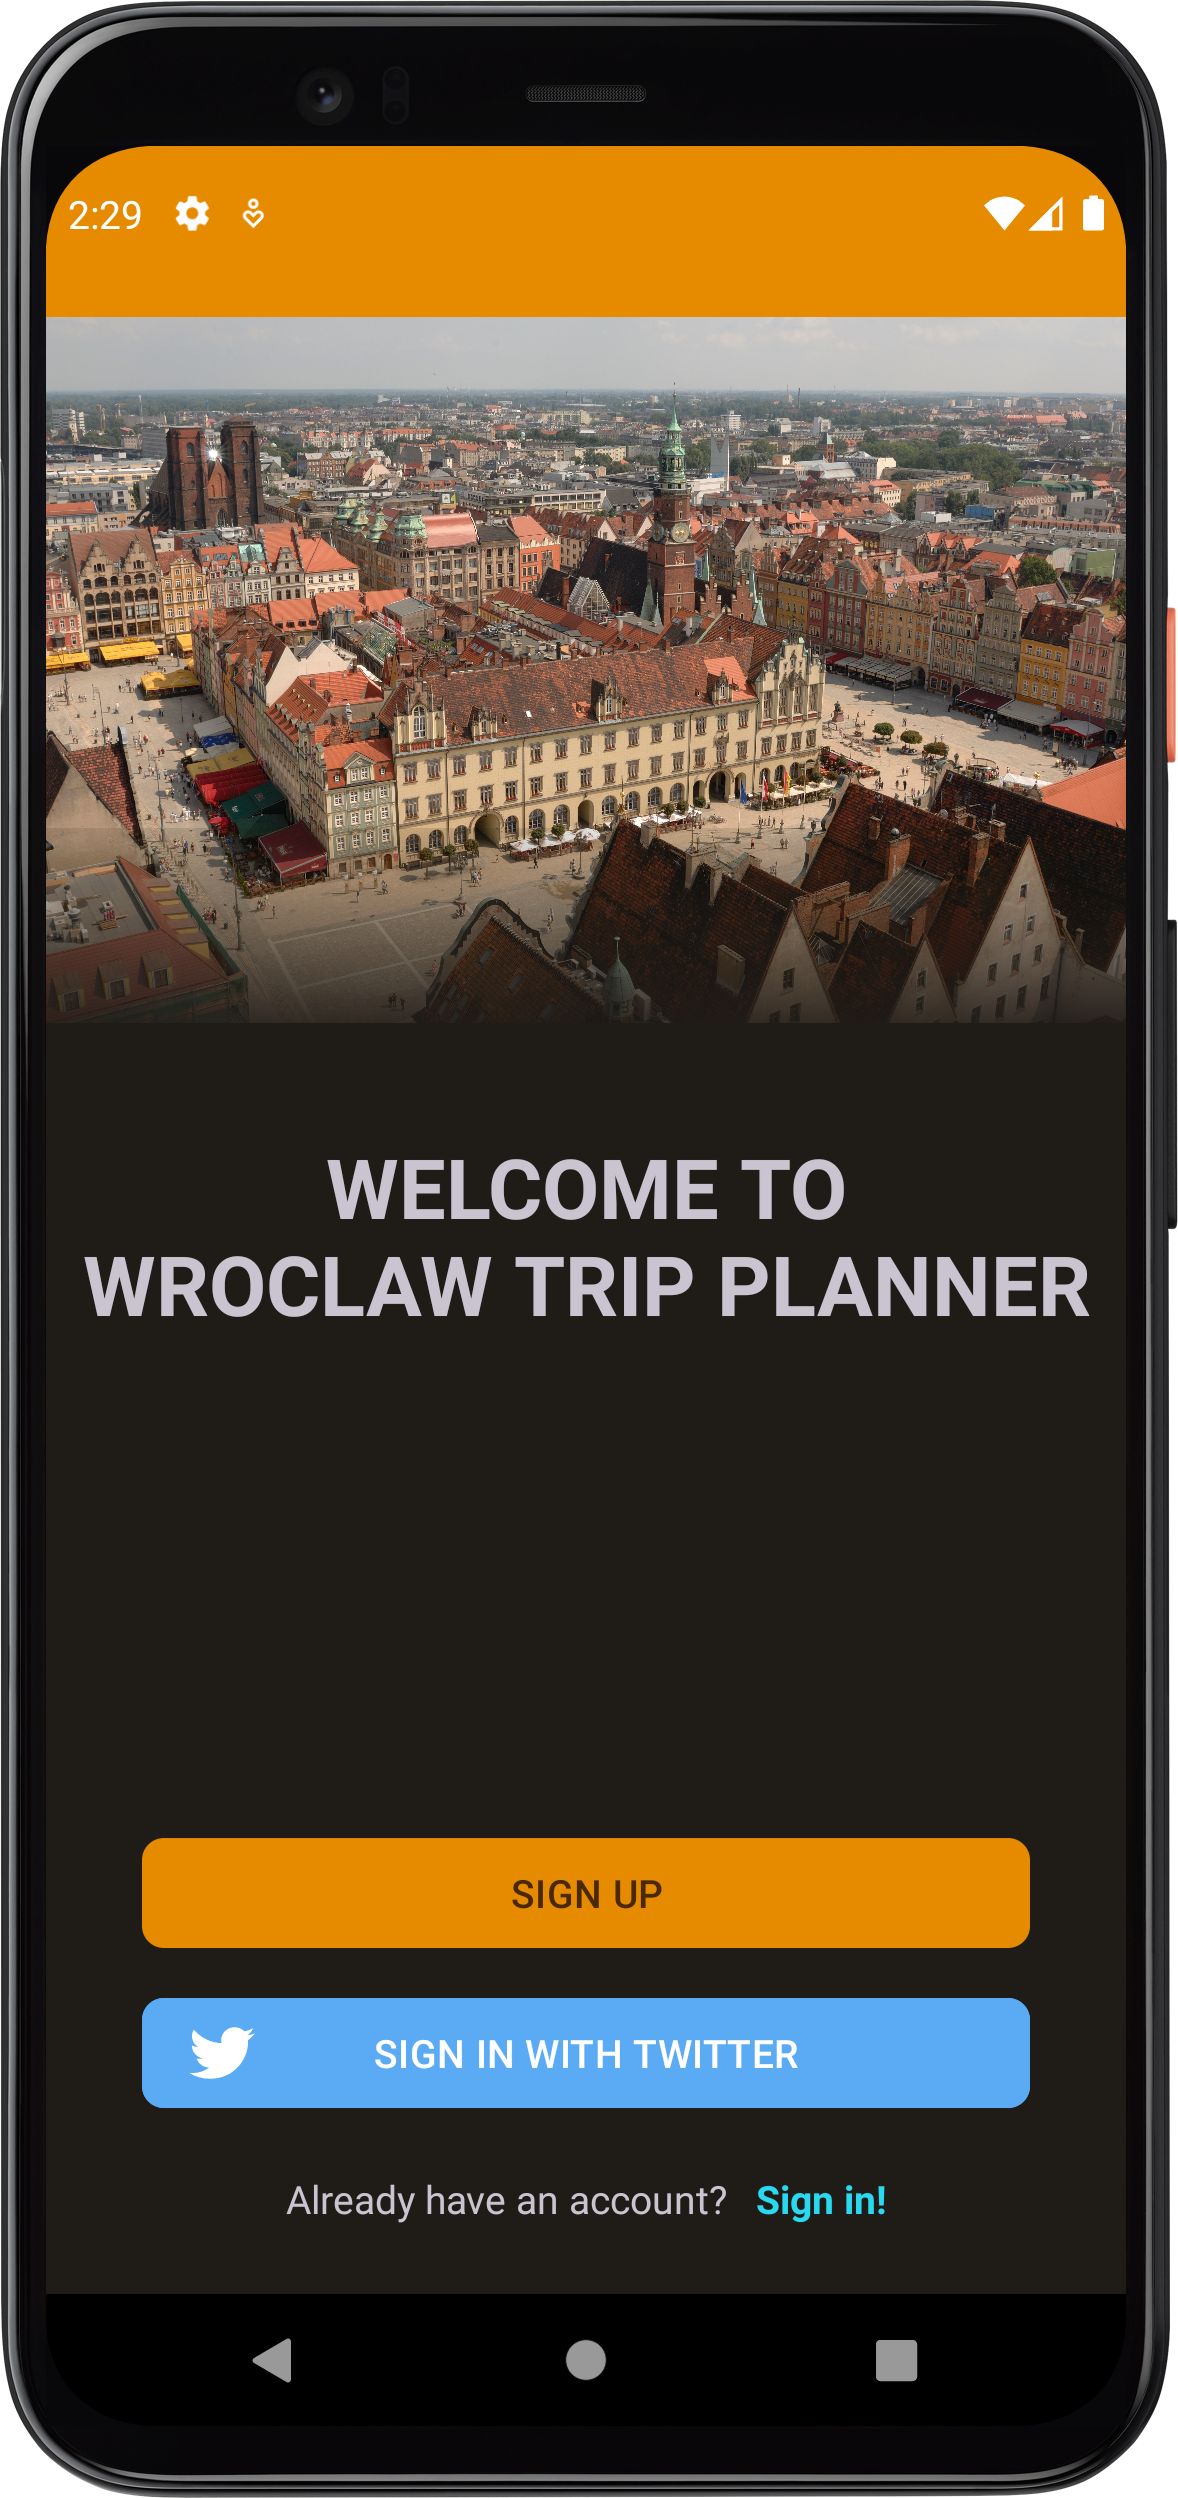
\includegraphics[scale=0.09]{src/app/welcome_fragment.png}
            \caption{Ekran powitalny aplikacji.\label{welcome}}
            \qquad
        \end{figure} 

        \subsubsection{Ekran rejestracji}
        Ekran rejestracji, widoczny na rysunku~\ref{register}, składa się przede wszystkim z pól tekstowych, do których użytkownik może wprowadzić pożądane informacje. Poprawność wprowadzanych danych jest
        w trakcie procesu rejestracji weryfikowana. Adres e-mail musi być odpowiednio sformatowany, pseudonim musi być unikalny, a hasło musi spełniać odpowiednie kryteria bezpieczeństwa. Poziom bezpieczeństwa
        hasła ukazywany jest za pomocą paska postępu, zaczerpniętego z biblioteki Material Design. Za pomocą kolorów i tekstu sygnalizuje on użytkownikowi to, czy hasło spełnia odpowiednie warunki. Aby móc
        utworzyć konto, hasło musi spełniać warunki opisane w instrukcji znajdującej się u dołu ekranu. Na samym dole znajduje się przycisk „REGISTER”. Wciśnięcie go powoduje weryfikację danych. W przypadku,
        jeśli któreś z pól wypełnione jest niepoprawnie, wyświetlane jest powiadomienie, a kursor użytkownika automatycznie przemieszcza się w wymagające uwagi pole.

        \vspace{1cm}
        \begin{figure}[!ht]%
            \centering
            \begin{subfigure}[b]{0.3\textwidth}
                \centering
                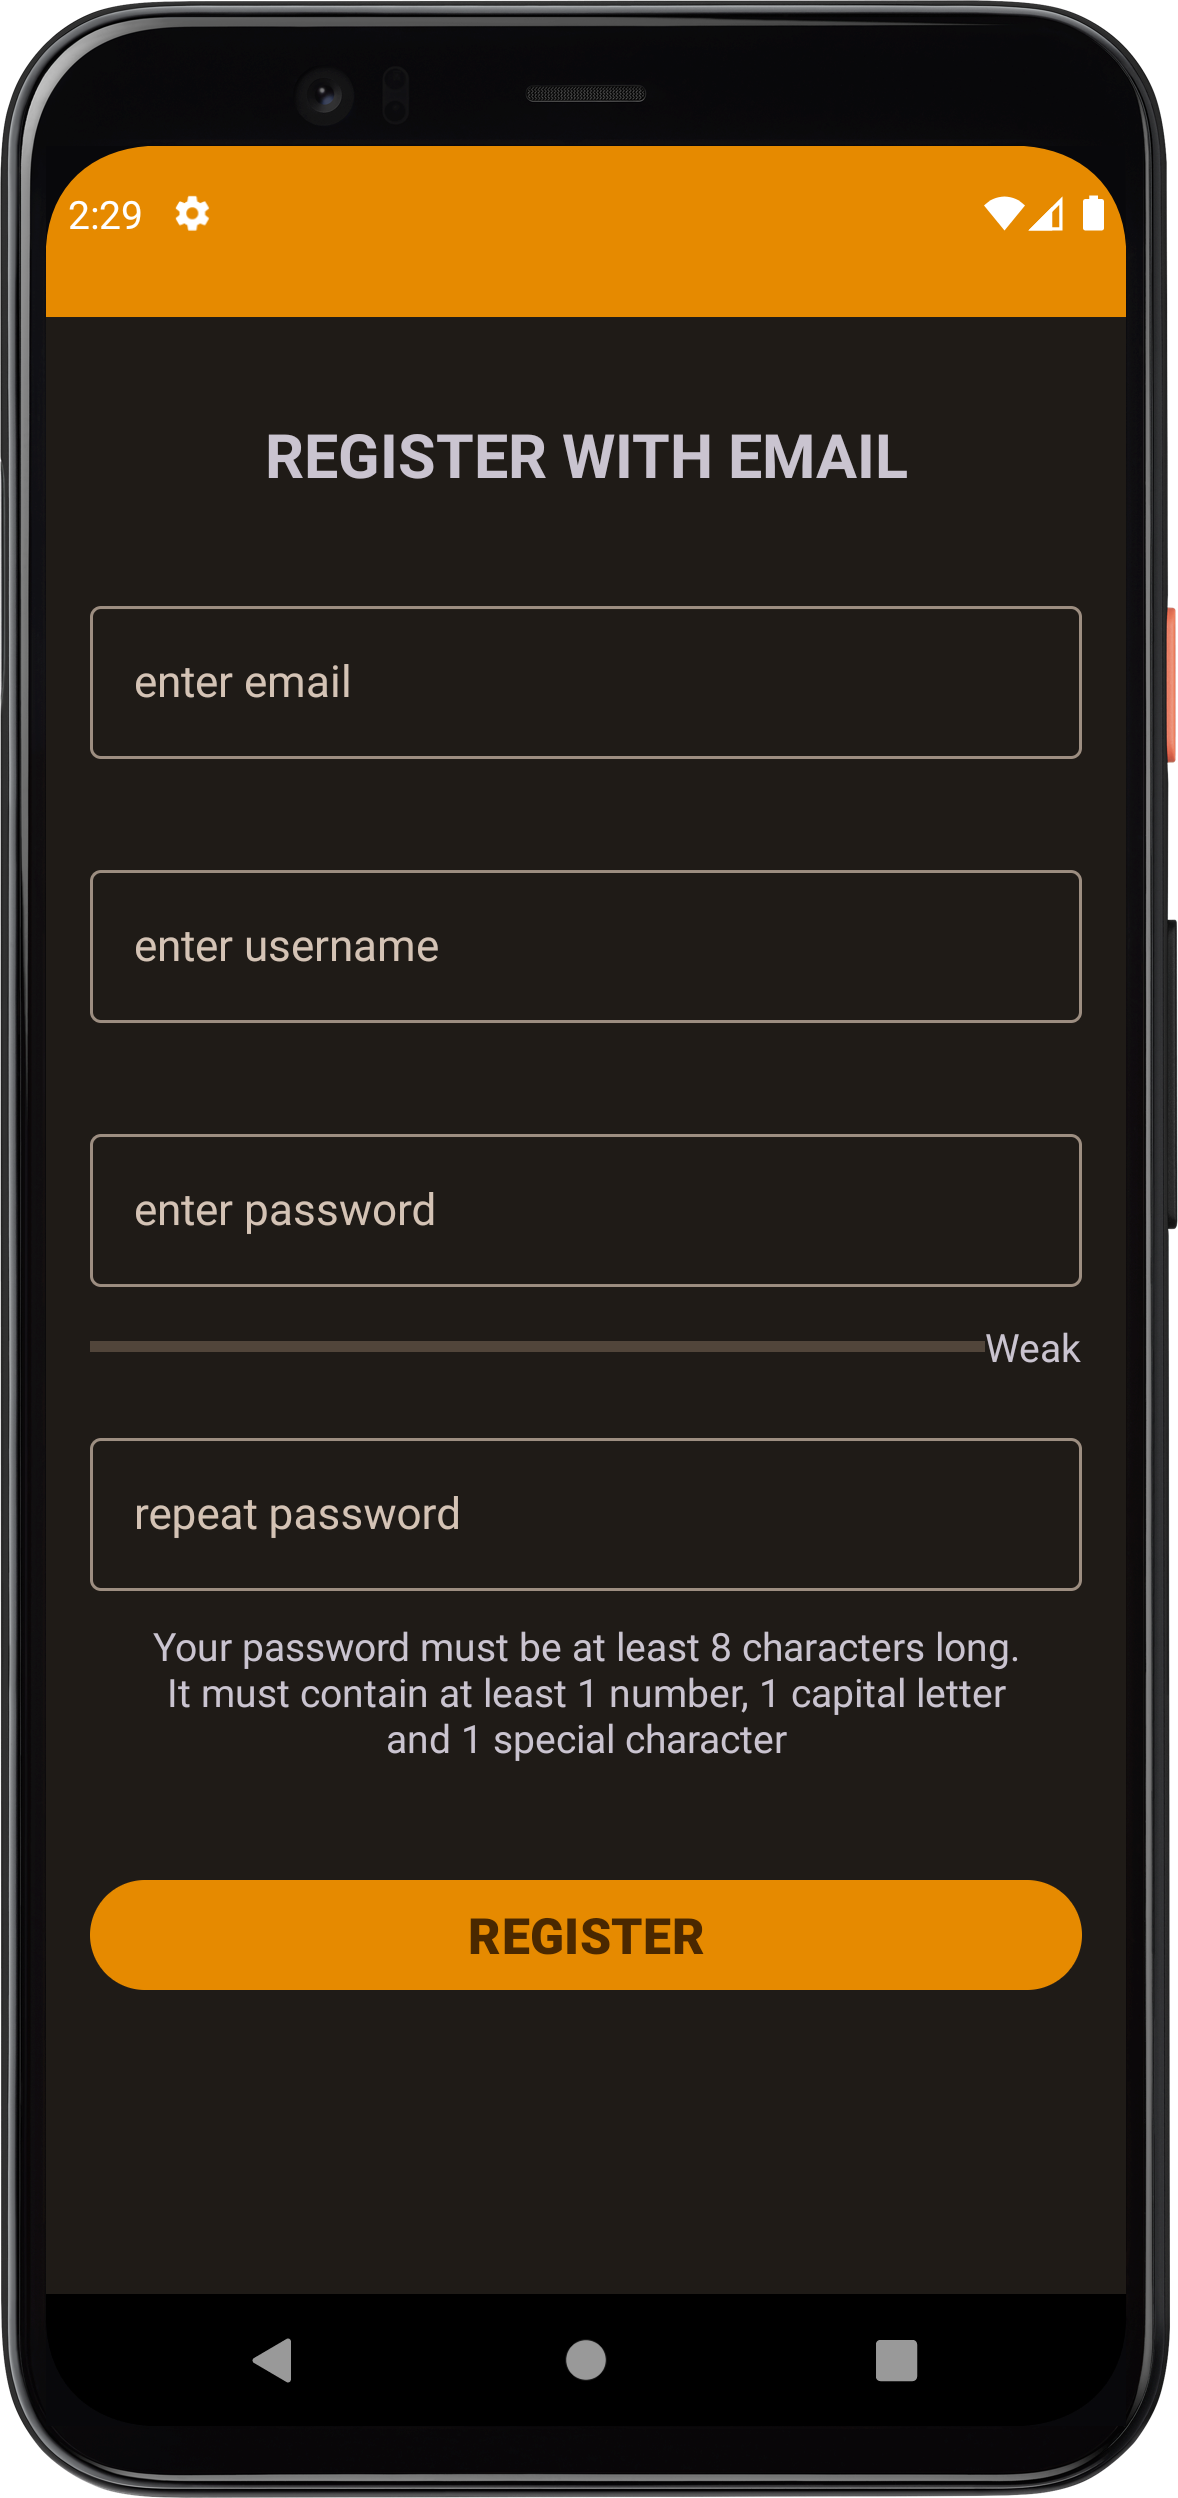
\includegraphics[width=\textwidth]{src/app/register1.png}
                \caption{Pusty ekran rejestracji.\label{register1}}
            \end{subfigure}
            \hfill
            \begin{subfigure}[b]{0.3\textwidth}
                \centering
                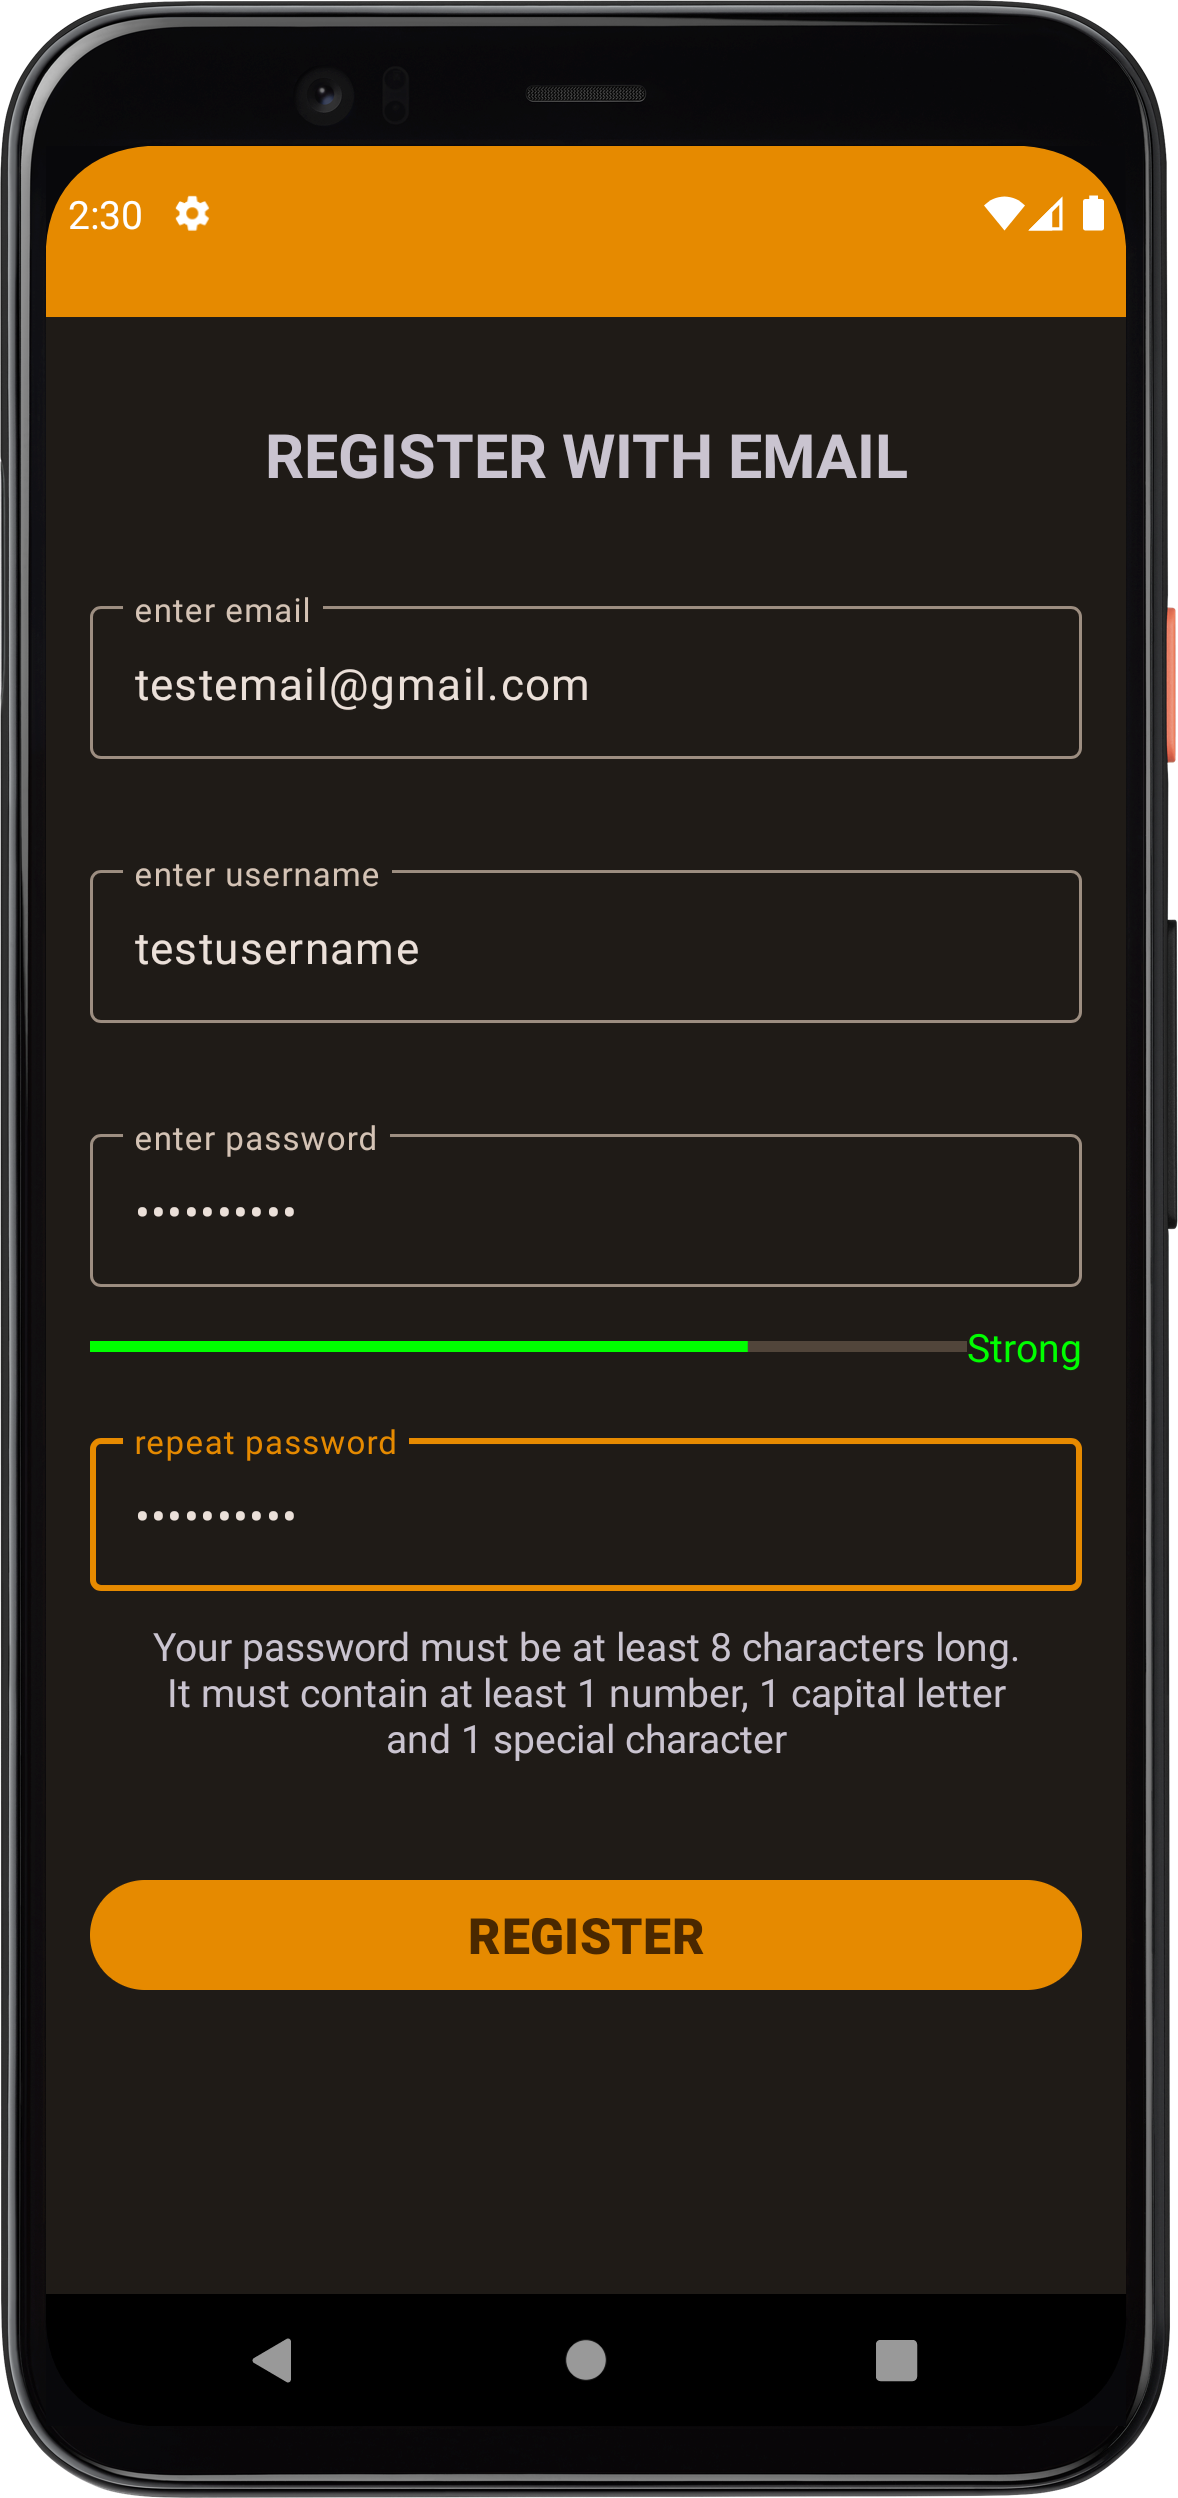
\includegraphics[width=\textwidth]{src/app/register2.png}
                \caption{Uzupełniony ekran rejestracji.\label{register2}}
            \end{subfigure}
            \caption{Ekran rejestracji użytkownika.\label{register}}
            \qquad
        \end{figure} 

        \subsubsection{Ekran logowania za pomocą konta Twitter}
        Użytkownik może uzyskać dostęp do aplikacji, logując się za pomocą konta Twitter. Reprezentujący tę opcję przycisk przekieruje użytkownika do przeglądarki, gdzie poproszony on zostanie o autoryzację
        dostępu aplikacji do konta Twitter (patrz rys.~\ref{twitter}). W obecnych czasach popularne jest oferowanie w aplikacjach mobilnych i internetowych opcji logowania za pomocą strony trzeciej, ponieważ
        wielu użytkowników może nie być chętnymi do tworzenia nowego konta w danym serwisie. Dodanie tego typu opcji niweluje ten problem, pozwalając użytkownikowi na korzystanie z konta istniejącego już w
        innym serwisie. Przy tego typu rejestracji pseudonim użytkownika z serwisu Twitter zostanie ustawiony jako pseudonim w aplikacji. W wypadku, jeśli pseudonim ten jest już zajęty, użytkownik zostanie
        poproszony o wybór nowego, unikalnego pseudonimu.

        \vspace{1cm}
        \begin{figure}[!ht]%
            \centering
            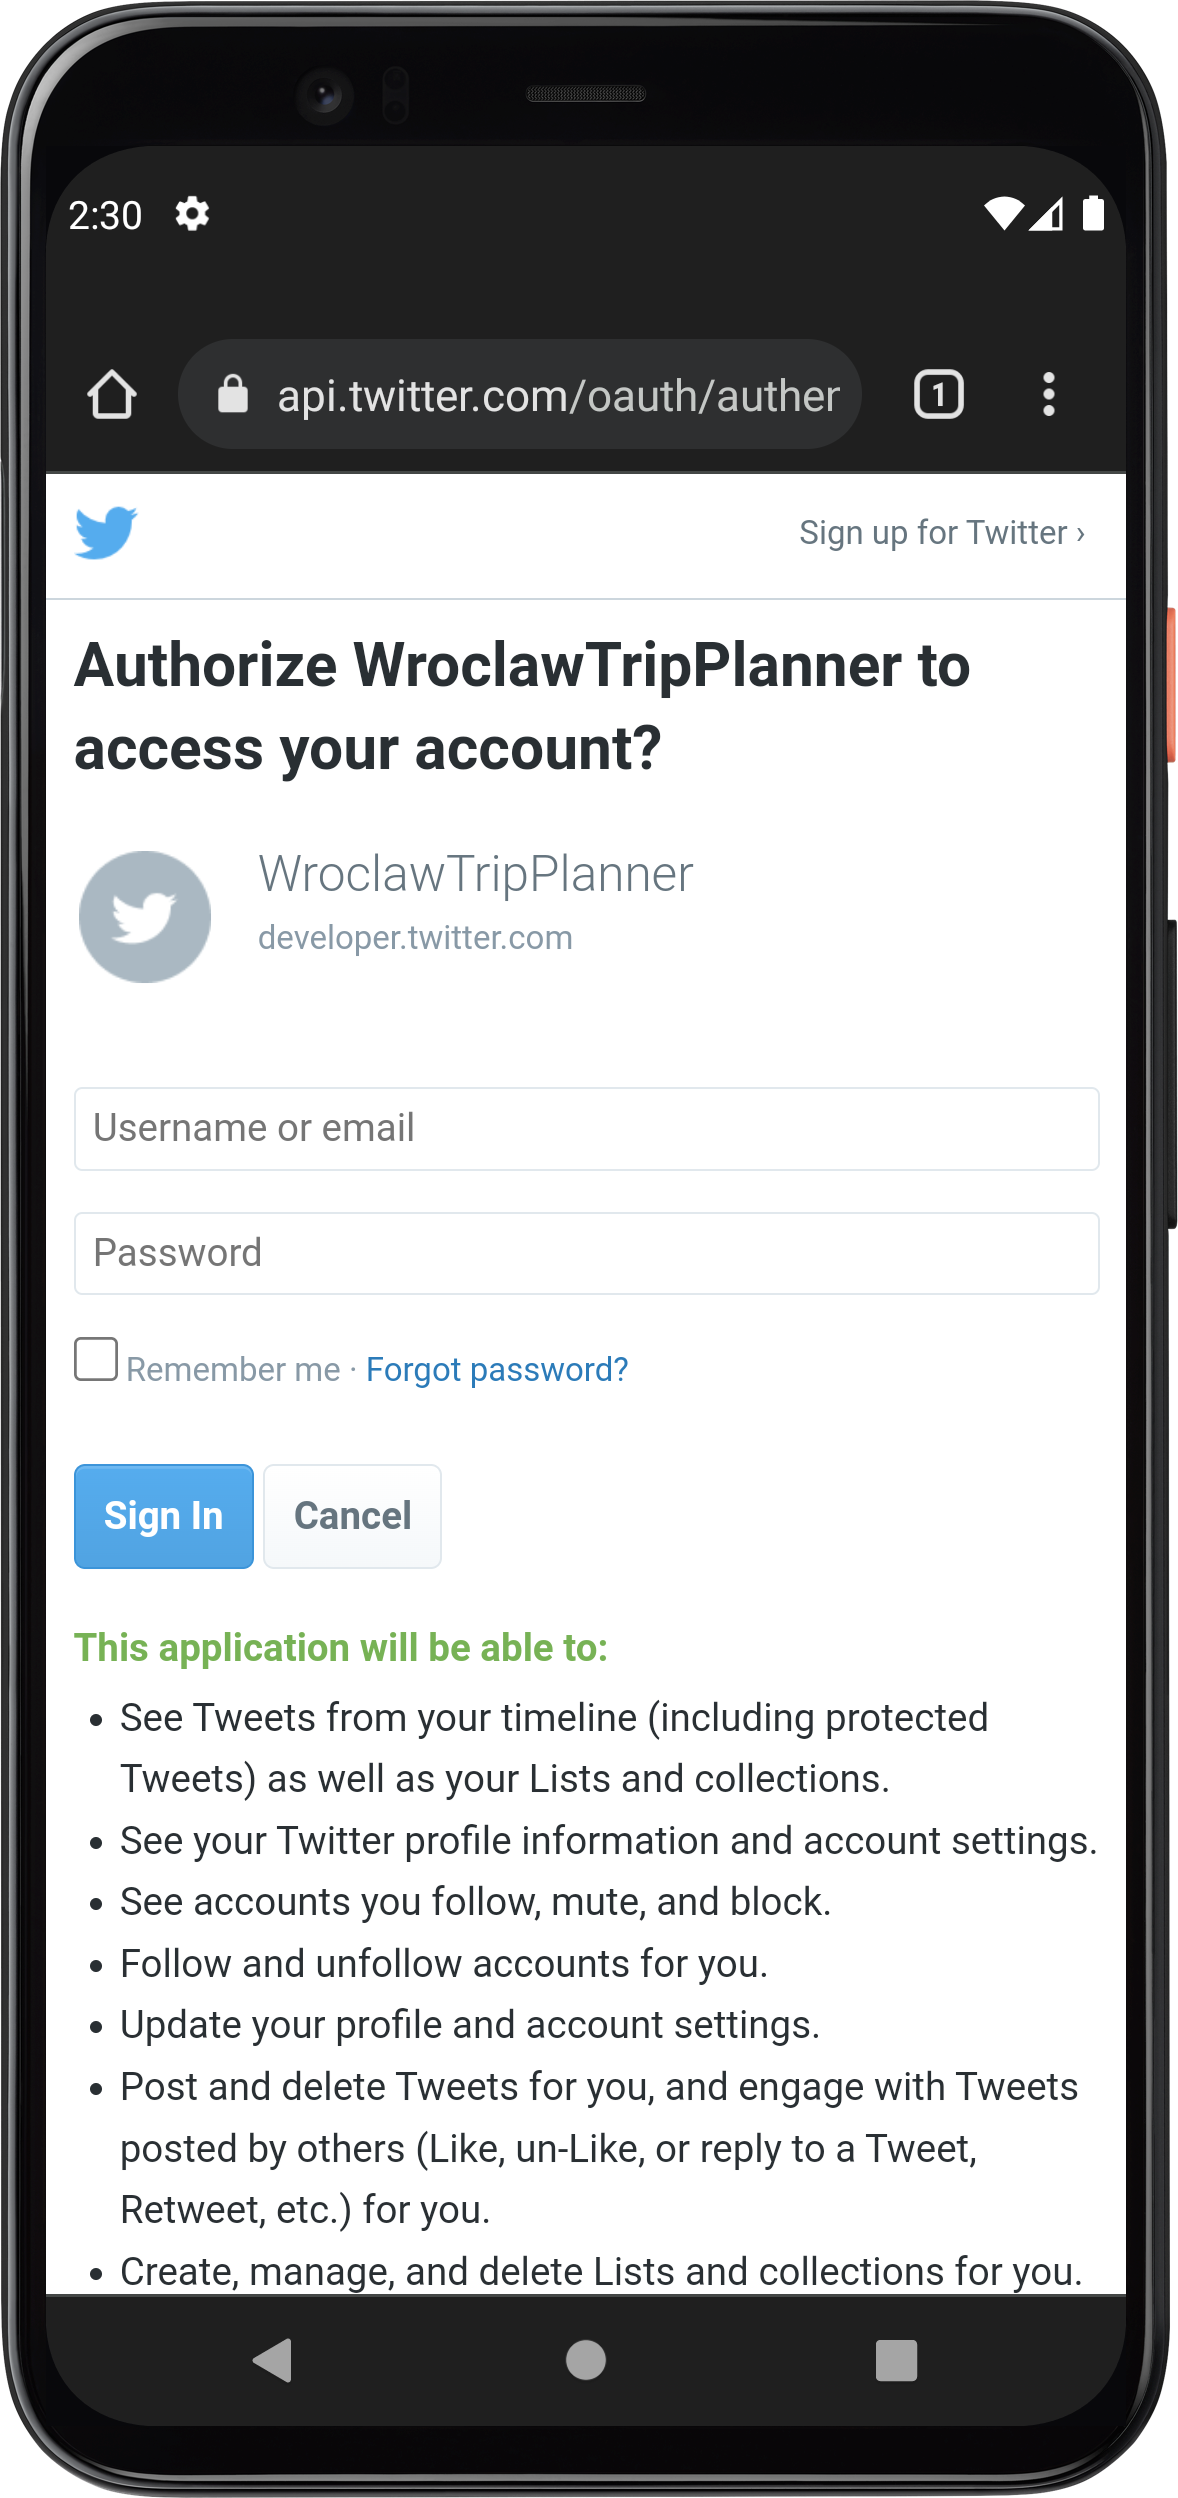
\includegraphics[scale=0.15]{src/app/twitter_login.png}
            \caption{Okno autoryzacji za pomocą konta Twitter.\label{twitter}}
            \qquad
        \end{figure} 